\chapter{Schülerinformationstag}

\section{Einleitung}

Der Schülerinformationstag wird jährlich durch das Department für Informatik der Universität Oldenburg veranstaltet und ist an informatik"=interessierte Schülerinnen und Schüler aus der Umgebung adressiert.
An Ständen sowie in Vorträgen werden den Interessierten Inhalte und Aufbau des Informatikstudiums in Oldenburg näher gebracht und interessante Projekte des Departments vorgestellt.
Im Jahr 2019 fand der Informationstag am 24. Januar unter dem Motto "`Informatik - KI und du!"' statt.
Im Rahmen dieser Veranstaltung bekam unsere Projektgruppe die Möglichkeit sich und das Projekt vorzustellen.
Dies haben wir mit zwei Angeboten genutzt:
Zum ersten haben wir unsere Vision in einem 30"=minütigen Vortrag präsentiert.
Zum anderen haben wir einen zweieinhalb"=stündigen Workshop veranstaltet, in dem angemeldete Schülergruppen zu zweit oder dritt einen Sensorknoten zusammenbauen und konfigurieren konnten.
Dieser wurde dann vorerst an der Universität in Betrieb genommen, um ihn später an den Schulen der teilnehmenden Schülerinnen und Schülern anzubringen.

Ziel der Teilnahme am Informationstag war es zum einen, Aufmerksamkeit und Interesse für unsere Projektgruppe zu erregen, aber vor allem, erste Standorte zur Anbringung von Sensorknoten zu gewinnen (vgl. \Fref{sec:SensorknotenLoesung}).

Bei der Vorbereitung und Durchführung der Präsentation und des Workshops haben sich vielfältige Aufgaben ergeben.
Neben der inhaltlichen Vorbereitung für den Zusammenbau des Sensorknotens durch die Schülerinnen und Schüler musste zuallererst ein Prototyp unseres Systems entwickelt werden, um ihnen eine angemessene Darstellung der Messwerte bereitzustellen.
Zusätzlich mussten allgemeine organisatorische Aufgaben bewältigt und insbesondere die Anmeldungen der teilnehmenden Schulen koordiniert werden.

\section{Teilnehmende Schulen}

Mit den Einladungen zum gesamten Informationstag gingen auch Informationen zu unserem angebotenen Workshop an die Schulen.
Für diesen Workshop mussten die Schulen sich mit Namen der Teilnehmenden offiziell bei der Projektgruppe anmelden.
Darüber hinaus haben wir noch einzelne Gruppen spontan nach dem Vortrag zu unserer Vision zugelassen.

Eine Ausbringung der Sensorknoten war leider nicht an allen teilnehmenden Schulen möglich. Dies lag zum Teil an fehlenden Rückmeldungen der Lehrkräfte, im Fall der Graf"=Anton"=Günter"=Schule an Bedenken des Landkreises Oldenburg (Schulträger).
Bei den übrigen Teilnehmern erfolgte die Anbringung zwischen Februar und April.

Folgende Schulen nahmen am Workshop teil.
In der Tabelle werden die Anzahl der zusammengebauten Sensorknoten je Schule (\#SK), die Art und das Datum der Anbringung aufgeführt.
"`Vor Ort"' bedeutet, dass Projektgruppenteilnehmer bei der Schule vor Ort waren, um ihn für das WLAN zu konfigurieren und anzubringen.
"`Abgabe"' bedeutet, dass der Sensorknoten an einen Vertreter der Schule übergeben wurde. \\

\begin{tabular}{|l|l|l|l|}
	\hline \textbf{Schule} & \textbf{\#SK} & \textbf{Anbringung} & \textbf{Datum} \\
	\hline Graf"=Anton"=Günter"=Schule & 2 & keine & - \\
	\hline Liebfrauenschule & 2 & vor Ort & 28.02.2019 \\
	\hline Herbartgymnasium & 2 & vor Ort & 26.03.2019 \\
	\hline Cäcilienschule Oldenburg & 1 & vor Ort & 20.06.2019 \\
	\hline IGS Kreyenbrück & 2 & keine & - \\
	\hline Cäcilienschule Wilhelmshaven & 1 & Abgabe & - \\
	\hline
\end{tabular}

\section{Prototyp}

Wie in der Einleitung angedeutet, musste für den Schülerinformationstag ein Prototyp des Sensorknotens sowie einer Webseite entwickelt werden, um den Schülerinnen und Schülern eine ansprechende Darstellung der Messwerte ihrer zusammengebauten Sensorknoten zu ermöglichen.
Als Grundlage für den Knoten diente hierbei das Projekt \textit{luftdaten.info} des \textit{OK Lab Stuttgart} \cite{luftdateninfo}.
Dieser sollte abgeändert werden, damit er die gemessenen Daten an eine eigens entwickelte IoT"=Plattform sendet, von der die Webseite ihre anzuzeigenden Daten abruft.
Ein Prototyp für eine Routingapplikation war zu diesem Zeitpunkt weder notwendig noch zielführend. Im Weiteren werden die Einzelkomponenten des Prototyps und deren Zusammenspiel genauer erläutert.

\subsection{Sensorknoten}

Eine weitere zentrale Komponente des Prototyps ist der Sensorknoten, welcher durch verschiedene Sensoren die Umweltdaten misst.
Diese gemessenen Werte werden anschließend den Schülern auf der Webseite zur Verfügung gestellt. Als Grundlage für den Sensorknoten wird der Stuttgart"=Sensor verwendet, der bereits auf luftdaten.info zum Einsatz kommt.
Der Sensorknoten von luftdaten.info kann in der Grundkonfiguration Feinstaubwerte der Größen pm2.5, sowie pm10 in \si{\mu g} pro \si{{m^3}} messen.
Als Sensor wird dazu der Nova Fitness SDS011 verwendet.
Dieser ist mit einen Mikrocontroller vom Typ ESP8266, hier auf einem Entwicklungsboard namens NodeMCU, verbunden.
Auf diesem läuft die Software (in diesem Kontext auch Firmware genannt) von luftdaten.info, die die Sensorik anspricht, und die Messdaten dann über das integrierte WLAN"=Modul des ESP8266 an die voreingestellten Server (von luftdaten.info und weiteren) überträgt.
Anpassungen an dem Verhalten der Firmware können beschränkt über ein Webinterface vorgenommen werden.
Dazu zählen unter anderem die WLAN"=Verbindungseinstellungen sowie die angeschlossene Sensorik.
Da die Messungen im Außenbereich stattfinden sollen, wird von luftdaten.info vorgeschlagen, die Komponenten in zwei \si{90^{\circ}}"=Kunststoffrohrbögen zu verbauen, um sie vor Nässe und anderen Umwelteinflüssen zu schützen.
Ebenfalls sollen die offenen Enden der Rohre mit Pflanzenschutzgitter versehen werden, um ein Eindringen von Ungeziefer vorzubeugen.

Da der in der Grundkonfiguration verwendete Feinstaubsensor SDS011 bei hoher Luftfeuchtigkeit ungenaue Werte liefert, wurde ein weiterer Umweltsensor, ein BME280 von Bosch, hinzugezogen, welcher ebenfalls von der Firmware unterstützt wird.
Damit kann die Temperatur, der Luftdruck und die relative Luftfeuchtigkeit der Umgebungsluft gemessen werden, um im späteren Verlauf des Projektes Korrelationen zu den Feinstaubwerten erarbeiten zu können.
Dieser Aufbau entspricht dem Sensorknoten, der an den Schulen angebracht wurde.

Da die o.g. Firmware nur beschränkt über das Webinterface angepasst werden kann, konnte sie in dem Zustand nicht für die IoT"=Plattform dieses Projektes verwendet werden.
Daher wurde ein Fork aus dem quelloffenen Repository von luftdaten.info gestartet, in dem die Integration mit der IoT"=Plattform dieses Projektes umgesetzt werden konnte.
Dazu wurden zuerst einige grundlegende Entscheidungen getroffen:

\begin{enumerate}
	\item Der Sensorknoten soll kompatibel zu luftdaten.info bleiben.
	\item Der Webserver vom Sensorknoten soll nur noch Messwerte anzeigen können.
	\item Die Konfiguration wird über die serielle Schnittstelle (USB) vorgenommen.
	\item Die Hardwareunterstützung wird auf die Hardware dieses Projektes reduziert.
	\item Integration der IoT"=Plattform dieses Projektes in die Firmware.
\end{enumerate}

Punkt 1 dient dazu, keine zusätzliche Konkurrenz zu schaffen.

Punkt 2 addressiert einige sicherheitstechnische Probleme der aktuellen Firmware.
Bisher kann jeder Netzwerkteilehmer den Sensorknoten (fehl"=)konfigurieren und sogar neu starten.
In einem öffentlichen Netzwerk, wie es bei einigen Schulen der Fall ist, muss diese Möglichkeit unterbunden werden.

Punkt 3 ist die Konsequenz aus Punkt 2 und minimiert das Risiko weiter, dass der Sensorknoten von Unbefugten manipuliert wird, da nun physischer Zugang zum Sensorknoten gegeben sein muss, um ihn zu konfigurieren.

Punkt 4 resultiert aus dem völlig unstrukturierten Quellcode von luftdaten.info (Stand Nov '18) und ermöglicht es, für dieses Projekt ungenutzten Code zu entfernen, um eine bessere Lesbarkeit, sowie Wartbarkeit zu erzielen.

In der Umsetzung erwiesen sich Punkte 1, 2 und 4 als trivial, da "nur" Code entfernt werden musste.
Diese Codestellen konnten unter Zuhilfenahme der Entwicklungsumgebung zuverlässig und schnell gefunden werden.
Punkt 5 konnte mit mäßigem Aufwand realisiert werden, da die Schnittstelle der IoT"=Plattform, ebenso wie die Schnittstelle von luftdaten.info, auf einer REST Architektur basiert, und somit nahezu direkt in den Code einfließen kann.
Die Autorisierung über JSON"=Web"=Tokens (JWT) konnte ebenfalls mit geringem Aufwand realisiert werden, da der Inhalt des Tokens nicht verarbeitet werden musste.
Die Aktualität des Tokens wurde darüber sichergestellt, dass vor dem Senden einer Messung jeweils ein neues Token angefordert wurde.
Punkt 3 hingegen erwies sich als Problem, da eine Konfiguration über die serielle Schnittstelle wenig anwenderfreundlich ist.
Daher wurde als Lösung sowohl die Schnittstelle selber implementiert, sodass ein erfahrener Anwender, unter Zuhilfenahme eines Terminals, den Sensorknoten konfigurieren konnte, als auch eine Graphische Benutzungsoberfläche entwickelt, die einen potentiellen Sensorknotenbetreiber durch die einzelnen Konfigurationsmöglichkeiten führt.
Die Reiter zum Aufspielen der Firmware, sowie zur Konfiguration des WLANs sind in \Fig{skItoolOldFirmware} und \Fig{skItoolOldWifi} zu sehen.

\begin{figure}[H]
	\centering
	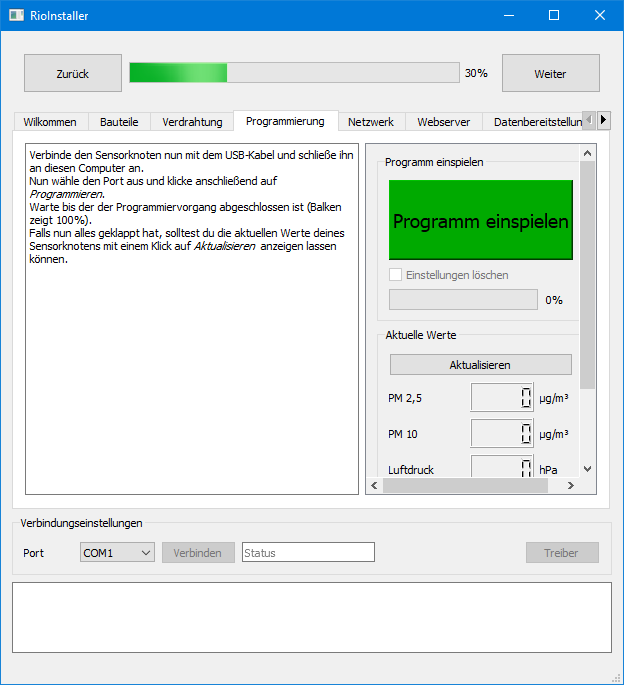
\includegraphics[width=\textwidth]{./ressourcen/Programmierung_neu.png}
	\caption{Reiter: Aufspielen der Firmware}
	\label{fig:skItoolOldFirmware}
\end{figure}

\begin{figure}[H]
	\centering
	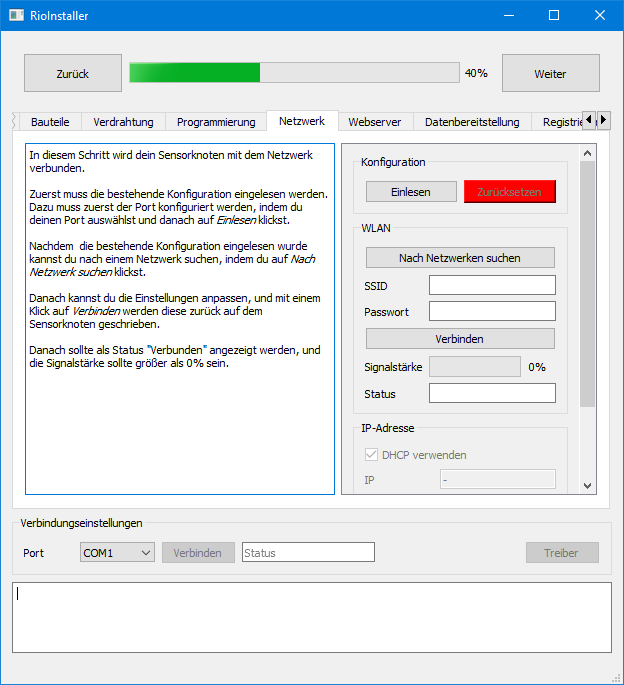
\includegraphics[width=\textwidth]{./ressourcen/Netzwerk_neu.png}
	\caption{Reiter: WLAN Konfiguration}
	\label{fig:skItoolOldWifi}
\end{figure}

Dieses Konfigurationstool wurde beim Schülerinformationstag und bei der Anbringung der Sensorknoten an den jeweiligen Schulen verwendet und erwies sich als ausreichend benuzerfreundlich, um den Sensorknoten in Betrieb zu nehmen.
Das dabei gesammelte Feedback soll daher im weiteren Verlauf des Projektes eingearbeitet werden, um das Konfigurationstool weiter zu verbessern.

\subsection{IoT"=Plattform}
Die im Rahmen des Schülerinformationstages entwickelte prototypische IoT"=Plattform ist die zentrale Schnittstelle zur Annahme und Bereitstellung der gemessenen Messdaten, der bereits im vorherigen Abschnitt beschriebenen Sensorknoten. \\
Für die prototypische Implementierung der IoT"=Plattform wurde die Technologie NodeJS im Zusammenspiel mit einer MongoDB als Datenspeicher eingesetzt.
Diese Entscheidung ist durch die einfache und schnelle Möglichkeiten der Technologien zur Entwicklung eines Prototypen und der bereits vorhanden Erfahrung innerhalb der Projektgruppe zu begründen.
Des Weiteren bietet NodeJS durch die Verwendung von JavaScript eine große Sammlung an bereits vorhanden Lösungen zu ähnlichen Problemen was die Entscheidung nur noch bekräftigt hat. \\
Die Hauptfunktionen der IoT"=Plattform sind dabei die Annahme der Messdaten von authentifizierten Sensorknoten, die Speicherung dieser und der anschließenden Bereitstellung für die Webseite, welche ebenfalls im Rahmen des Schülerinformationstages implementiert wurde.
Um diese Hauptfunktionen zu realisieren wurde ein HTTP"=Server mit spezifischen Endpunkten zur Authentifizierung, Annahme und Bereitstellung der Messdaten implementiert.
Des Weiteren kommt die bereits genannte Datenbank MongoDB zum Einsatz für die dauerhafte Speicherung der Mess- und Nutzerdaten. \\
Zur Authentifizierung an der IoT"=Plattform wird der OAuth2.0 Standard verwendet.
Dieser erlaubt eine sichere und einfache Authentifizierung von Nutzern der IoT"=Plattform, welche im Falle des Schülerinformationstages die Sensorknoten und Webseite sind.
Vom Standard wird der Client Credentials Flow verwendet, welche den Nutzern erlaubt Benutzername und Passwort für ein JSON Web Token auszutauschen, welches zur Bereitstellung von neuen Messdaten oder der Abfrage von Bestehenden verwendet werden kann. \\
Die Schnittstelle zur Annahme von Messdaten ist nur für Sensorknoten verwendbar, was mit Hilfe des übergebenen JSON Web Token überprüft wird.
Der Sensorknoten übermitteln bei der Schnittstelle per HTTP POST ihre aktuelle Position und die gemessenen Messdaten, welche nach einer Validierung in der Datenbank gespeichert werden. \\
Damit die im Schülerinformationstag entwickelte Webseite die vorhanden Messdaten anzeigen kann wurde die Schnittstelle zur Bereitstellung der Messdaten implementiert.
Dabei kann die Webseite über gesonderte Schnittstellen alle Messdaten aller Sensorknoten, alle Messdaten eines speziellen Sensorknoten und alle Messdaten eines speziellen Sensorknoten, welche in einem bestimmten zeitlichen Intervall liegen, abfragen.  

\subsection{Webseite}

Eine weitere wichtige Komponente des Schülerinformationstages ist das Frontend, beziehungsweise die Webseite, mit dem Ziel, die gemessenen Daten live anzeigen zu können.
Das dabei entwickelte Frontend soll weiterhin für die Schulen und Schüler zur Verfügung stehen, damit diese auch nach dem Schülerinformationstag und der Anbringung der Sensoren ihre gemessenen Daten einsehen und ggf. analysieren können.
Um dieses Ziel zu erreichen haben wir uns für eine Webseite mit dem Angular"=Framework entschieden, was zum größten Teil mit den bereits vorhandenen Erfahrungen innerhalb der Projektgruppe zusammenhängt, da mehrere Mitglieder bereits mit diesem Framework gearbeitet haben und die Vorbereitungszeit sehr begrenzt war.
Um den Schülerinnen und Schülern eine ansprechende Darstellung der Werte zu liefern, haben wir uns für eine Visualisierung der Daten als Diagramm, welches durch Highcharts unterstützt wird, entschieden.
Dabei handelt es sich um ein Plugin, welches auf Javascript basiert und das angezeigte Diagramm anhand von verschiedener Datensätze anzeigen kann.
Außerdem wird die Darstellung der HTML"=Elemente durch die Bootstrap"=Bibliothek unterstützt.

\begin{figure}[H]
	\centering
	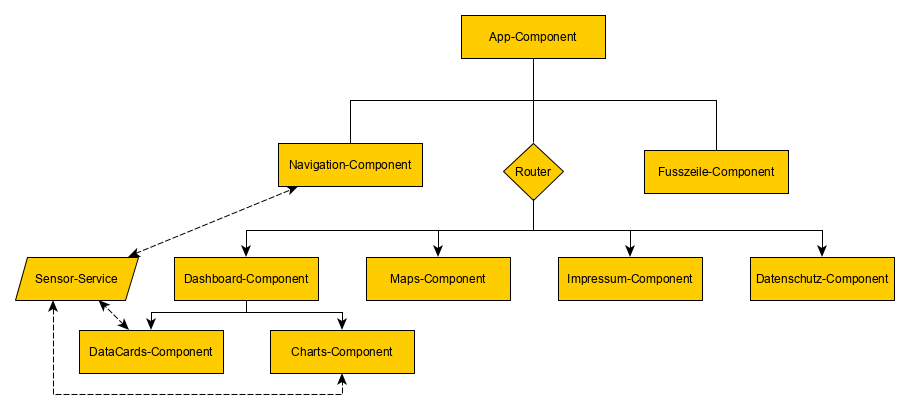
\includegraphics[width=\textwidth]{./ressourcen/schit-aufbau-frontend.png}
	\caption{Grundaufbau der Webseite}
\end{figure}

Die dabei entwickelte Applikation ist aus verschiedenen Komponenten aufgebaut.
Eine Komponente besteht aus einer HTML, einer SCSS und einer Typescript"=Datei.
Der Kern der Komponenten ist die App"=Komponente.
In dieser werden alle anderen Ansichten rein geladen.
Der Navigations- und der Fußzeilenbereich werden durchgehend angezeigt.
Die anderen Komponenten werden durch den Router in der Mitte der Applikation geladen. 

\begin{figure}[h]
	\centering
	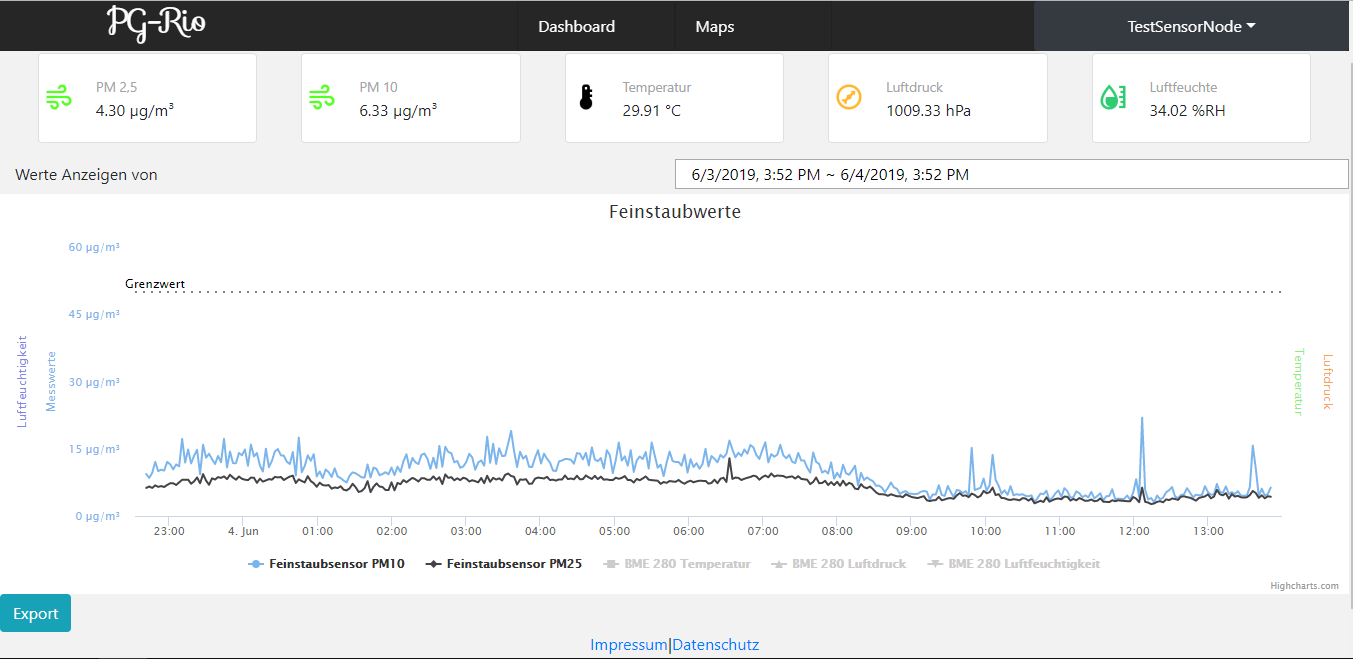
\includegraphics[width=\textwidth]{./ressourcen/schit-dashboard-frontend.png}
	\caption{Dashboard der Webseite}
\end{figure}

Beim ersten Aufrufen der Applikation wird auf die Dashboard"=Komponente weitergeleitet.
Diese bekommt dabei ihre Informationen von dem Sensor"=Service, welcher für die Kommunikation mit der IoT"=Plattform zuständig ist.
Er lädt die Daten von den ausgewählten Sensoren und bereitet sie für die Data"=Cards und das Diagramm auf.
Die Daten werden zu Beginn für den heutigen Tag geladen.
Um die Daten anderer Tage einzusehen, kann durch einen Kalender oberhalb des Charts ein anderer Zeitbereich ausgewählt werden, sodass auch ganze Wochen eingesehen werden können.
Im unteren Bereichs der Chart"=Komponente gibt es eine Möglichkeit, die Daten, die derzeit im Chart angezeigt werden, als CSV"=Datei zu exportieren.
Dabei werden die Sensordaten mit einem Zeitstempel im Unixformat versehen. 

Die Maps"=Komponente ist zur Darstellung der einzelnen Sensoren auf einer Map.
Diese wurden von uns händisch in den Kalender eingetragen.
Außerdem besitzen wir noch ein Impressum und eine Datenschutz"=Seite, um alle relevanten Nutzerdaten bereitzustellen. 


\subsection{Infrastruktur}
Eine weitere zentrale Komponente des Prototyps ist die Infrastruktur.
Um die Messdaten der verteilten Sensorknoten an eine zentrale Stelle senden zu können, diese dort entgegenzunehmen und zu speichern, sind über das Internet erreichbare Server nötig, die diese Dienste bereitstellen.
Des Weiteren muss den Schülerinnen und Schülern der Zugang zu der Webseite zum Anzeigen der gespeicherten Sensordaten über das Internet ermöglicht werden.
Für die Umsetzung dieser Anforderungen hat die Universität Oldenburg Ressourcen zur Nutzung von virtuellen Rechnersystemen (VMs) zur Verfügung gestellt.
In \Fref{fig:schitInfra} ist in einen Netzwerkdiagramm die dafür entwickelte und umgesetzte Infrastruktur für den Schülerinformationstag mit den drei folgenden verwendeten VMs dargestellt:
\begin{itemize}
\item \url{pg-rio-dvlp.Informatik.Uni-Oldenburg.DE} (Entwicklungsserver)
\item \url{pg-rio.Informatik.Uni-Oldenburg.DE} (Produktivserver)
\item \url{pg-rio-strg.Informatik.Uni-Oldenburg.DE} (Fileserver)
\end{itemize}
\newpage
\begin{figure}[H]
	\centering
	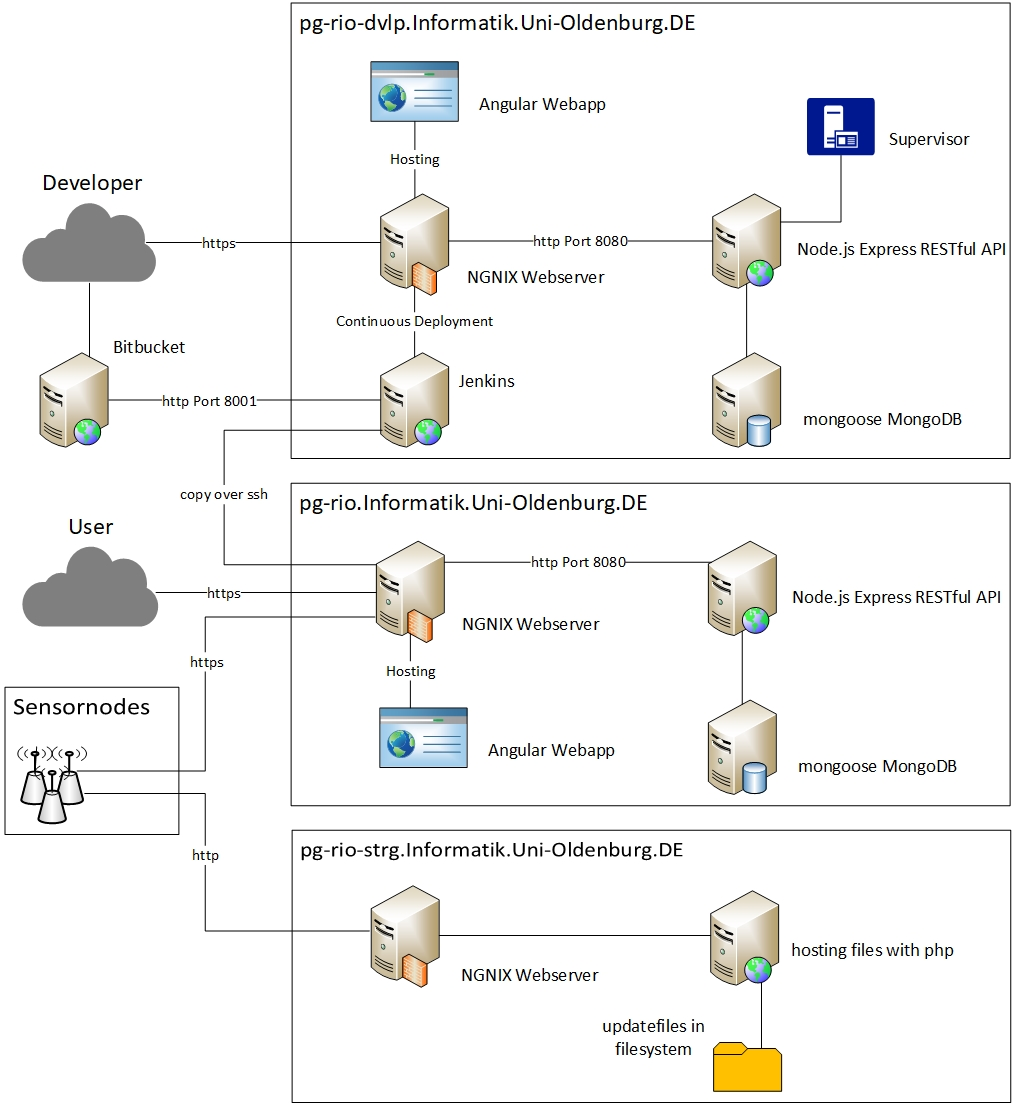
\includegraphics[width=\textwidth]{./ressourcen/SCHIT-Infrastruktur.jpg}
	\caption{Infrastruktur für Schülerinformationstag}
	\label{fig:schitInfra}
\end{figure}
\noindent
Im Folgenden werden die Funktionen der einzelnen Komponenten im Netzwerksdiagramm in \Fref{fig:schitInfra} erläutert:
\begin{itemize}
\item	\textbf{NGINX Webserver}\\
Die Webserver fungieren auf allen drei VMs als Reverse"=Proxy.
Die Aufgabe eines Reverse"=Proxy ist die Zugangskontrolle bei öffentlichen Anfragen über das Internet.
Des Weiteren werden dort die Anfragen zentral protokolliert.
Weitere Aufgaben der Webserver sind die Erreichbarkeit über das Internet mit einer gesicherten Verbindung über https zu ermöglichen, sowie die Webseite über den Entwicklungsserver und den Produktivserver zu veröffentlichen.     
\item	\textbf{Node.js Express RESTful API}\\
Die API ist für die Entgegennahme der Messdaten der Sensorknoten, dem Speichern der Messdaten in eine MongoDB, sowie dem Bereitstellen angefragter Messdaten über die Webseite zuständig.
Auf dem Entwicklungsserver läuft der Dienst in einen Supervisor.
Dieser ermöglicht in der Entwicklungsphase bei auftretenden Fehlern das Protokollieren der Fehlermeldungen, sowie das automatische Neustarten des Dienstes.
\item	\textbf{Jenkins}\\  
Der Jenkins"=Dienst auf dem Entwicklungsserver ermöglicht schnelle Aktualisierungen der Webseite in der Entwicklung.
Dazu ist dieser mit dem Bitbucket"=Dienst der Universität Oldenburg gekoppelt und führt bei Versionsaktualisierungen und Fehlerbehebungsmaßnahmen automatisch Kompiliervorgänge durch und veröffentlicht  aktualisierte Webseitenversionen.
\item	\textbf{Bereitstellung von Updatedateien}\\
Auf dem Fileserver werden Updatedateien für die Sensorknoten über einen php"=Dienst bereitgestellt.     
\end{itemize}

\subsection{Migration}
Am 11. September 2019 wurden die Sensorknoten mit der prototypischen Firmware des Schülerinformationstags auf den Stand der Neuentwicklung migriert und so in das neuentwickelte Produktivsystem eingebunden.
Dazu gibt es eine Migrationsfirmware, die auf dem Updateserver des alten Systems bereitgestellt wurde.
D.h. nur die Sensoren mit der prototypischen Firmware aktualisieren sich auf diese Migrationsfirmware.

Die Migrationsfirmware führt nacheinander folgende Schritte durch:

\begin{enumerate}
	\item Die Konfiguration der alten Firmware wird von \filename{config.json} in \filename{config.old.json} umbenannt.
	\item Die Standardkonfiguration für die neue Firmware wird in die Datei \filename{config.json} geschrieben.
	\item Die Datei \filename{credentials.json} wird durch mehrere Bausteine erzeugt.
	Darin enthalten sind die WLAN"=Zugangsdaten sowie die Zugangsdaten für die IoT"=Plattform aus der alten Konfiguration.
	\item Die mitgelieferte neue Sensorknoten"=Firmware wird in eine Datei auf dem Dateisystem geschrieben.
	\item Das Update wird mit der geschriebenen Update"=Datei durchgeführt.
	\item Die Update"=Datei wird gelöscht und das System neugestartet.
\end{enumerate}

Vorbereitend für die Migration wurden die Zugangsdaten der alten IoT"=Plattform in das neue System übertragen.
Nachdem die Migrationsfirmware hochgeladen wurde, konnten alle betroffenen und erreichbaren Sensorknoten innerhalb von 24 Stunden erfolgreich in das neue System migriert werden.

\section{Fazit}

Zum Abschluss des Berichts zur Teilnahme am Schülerinformationstags soll in Hinblick auf die Erreichung der angestrebten Ziele nun abschließend Bilanz gezogen werden.
Das war zum einen die Erregung von Aufmerksamkeit und zum anderen der Gewinn von Standorten zur Anbringung erster Sensorknoten.
Da im Rahmen des Informationstags nur wenige angebracht werden konnten, muss man in diesem Punkt von einem schlechten Ergebnis sprechen, das den aufgebrachten Aufwand nicht rechtfertigen kann.
Was allerdings die Erregung von Aufmerksamkeit betrifft, so konnten wir zumindest bei unseren Zuhörern und Teilnehmern ein großes Interesse an der verwendeten Technologie sowie der Feinstaub"=Thematik feststellen.
Das widerum gibt Anhaltspunkte für die Planung weiterer Maßnahmen zur Gewinnung von Sensorstandorten in späteren Projektphasen, die es gezielt zu planen gilt.
Denkbar wäre beispielsweise das Angebot weiterer Workshops für z.B. andere Studenten oder umweltbewusste Oldenburger.

Neben den gesetzten Zielen, müssen aber auch die gewonnen Erkenntnisse aus der Entwicklung des Prototyps bewertet werden.
So haben wir einerseits einen Teil Umsetzbarkeit unserer Vision gezeigt, aber auch eine Grundlage zur notwendigen Datenanalyse geschaffen.
Auch bei der Anforderungserhebung konnte der Prototyp helfen, erste Erkenntnisse als Basis zu nutzen.
In der Entwicklung konnten wir bereits vor Beginn der Hauptentwicklungsphase feststellen, wo wir unsere Zusammenarbeit im Team verbessern müssen.
Daher wollen wir ein besonderes Augenmerk darauf setzen, dass wir Wissensinseln vermeiden und die Synchronisation zwischen Teilteams geplant sicherstellen.

Unter Einbezug der erweiterten Erkenntnisse über die gesetzten Ziele hinaus bewerten wir die Teilnahme am Schülerinformationstag daher insgesamt als gelungen und zufriedenstellend.
